\documentclass[t]{beamer}
\usepackage[utf8]{inputenc}
\usepackage[english]{babel} % Untuk menyesuaikan format bibtex
\usepackage{natbib} % Untuk mengedit bibliografi (daftar)
\usetheme{Madrid}
\usepackage{graphicx}
\usepackage{hyperref}
\usepackage{multicol, multirow, tabularx}
\usepackage[compatibility=false]{caption}
\usepackage{subcaption}
\setbeamertemplate{caption}[numbered]
\addto\captionsenglish{\renewcommand{\figurename}{Gambar}}
\addto\captionsenglish{\renewcommand{\tablename}{Tabel}}
\title{Seminar Hasil Tugas Akhir}
\subtitle{PERANCANGAN PREPROCESSOR PADA SISTEM PENDETEKSI INTRUSI SNORT BERBASIS CONVOLUTIONAL NEURAL NETWORK DAN LONG SHORT TERM MEMORY}
\author{Didik Hadumi Setiaji}
\institute{
Jurusan Teknik Elektro\\
Fakultas Teknik\\
Universitas Mataram
}
\AtBeginSection[]
{\begin{frame}
\tableofcontents[currentsection]
\end{frame}
}
\begin{document}
\begin{frame}
	\titlepage
\end{frame}
\section{Pendahuluan}
\subsection{Rumusan Masalah} \label{rumusanmasalah}
\begin{frame}{Rumusan Masalah}
	Dari latar belakang dapat dirumuskan masalah sebagai berikut:
	\begin{enumerate}
		\item Bagaimana merancang profiling preprocessor sistem pendeteksi intrusi snort dengan metode Long Short Term Memori ?
		\item Bagaimana merancang filtering preprocessor sistem pendeteksi intrusi snort dengan metode Convolutional Neural Network ?
		\item Bagaimana merancang preprocessor sistem pendeteksi intrusi snort dengan kinerja yang optimal ?
	\end{enumerate}
\end{frame}
\subsection{Batasan Masalah}
\begin{frame}
	\frametitle{Pendahuluan | Batasan Masalah}
	Batasan masalah yang diterapkan pada penelitian ini adalah sebagai berikut :
	\begin{enumerate}
		\item Sistem yang dirancang berbasis \textit{service daemon} atau berjalan di belakang
		\item Sistem diujikan pada jaringan kabel \textit{ethernet} dengan skala jaringan LAN
		\item Sistem diujikan dengan menonaktifkan seluruh rule yang ada pada Snort IDS
		\item Pengujian sistem bersifat aktif atau disengaja
		\item Pendeteksian diujikan pada file malware yang sudah di \textit{training}.
	\end{enumerate}
\end{frame}
\subsection{Tujuan}
\begin{frame}{Tujuan}
	Berdasarkan latar belakang dan rumusan masalah, tujuan dari penelitian ini adalah sebagai berikut :
	\begin{enumerate}
		\item Dapat meningkatkan kapabilitas sistem pendeteksi intrusi snort dengan mengintegrasikan sistem \textit{deep learning} berupa CNN dan LSTM dalam pada sistem pendeteksi intrusi malware
		\item Menemukan arsitektur dan karakteristik model \textit{Deep Learning} yang optimal dijadikan sebagai metode pendeteksi intrusi malware
	\end{enumerate}
\end{frame}
\subsection{Manfaat}
\begin{frame}{Pendahuluan | Manfaat}
	\begin{enumerate}
		\item Memberikan kemudahan dalam pendeteksian intrusi \textit{malware} dengan snort IDS
		\item Menjadi referensi untuk mengimplementasikan metode \textit{Deep Learning} pada Snort IDS. Dapat menjadi acuan dari penelitian tentang bagaimana pengaruh dan manfaat penerapan metode \textit{deep learning}
	\end{enumerate}
\end{frame}
\section{Tinjauan Pustaka dan Landasan Teori}
\subsection{Tinjauan Pustaka}
\begin{frame}{Tinjauan Pustaka}
	\par Pada Penelitian \cite{zhang2001hide}, pengujian dilakukan dengan menggunakan beberapa jenis neural network antara lain Perceptron, Backpropagation, PBH, Fuzzy ARTMAP, dan Radial-based Function.
	\par Akurasi tertinggi dicapai oleh Backpropagation, dan PBH (Perceptron Backpropagation Hybrid), dimana MSR errornya berkurang seiring dengan jumlah data yang dimasukkan yang berkisar di 5\% sampai 10\% dari intensitas data background.
\end{frame}
\begin{frame}{Tinjauan Pustaka}
	\par Pada penelitian \cite{wirawan2015penerapan}, tentang penerapan kecerdasan buatan pada IDS.Penelitian ini menggunakan salah satu metode Machine Learning yakni Naive Bayes memperoleh akurasi sebesar 89\% dengan running time. Penelitian ini menerapkan \textit{Naive Bayes Classifier} dengan memilah atribut berdasarkan korelasi, dan menggunakan mean/standar deviasi untuk atribut kontinyu pada 3-interval dan 5-interval. Metode ini memperoleh akurasi sebesar 89\% dengan running time rata-rata 31 detik.
\end{frame}
\begin{frame}{Tinjauan Pustaka}
	\par Pada Penelitian \cite{jacobus2014penerapan}, tentang penerapan metode Support Vector Machine pada Intrusion Detection System secara Realtime menerapkan 3 kelas untuk proses pendeteksian jenis intrusi yakni normal, probe, dan DoS. Untuk beberapa tipe intrusi dapat terdeteksi dengan akurasi diatas 90\%, dengan memanfaatkan kluster pada beberapa jenis faktor parameter dari header packet yang diperoleh dari hasil data mining.
\end{frame}
\subsection{Landasan Teori}
\begin{frame}{Protocol Data Unit}
	\begin{figure}[H]
		\centering
		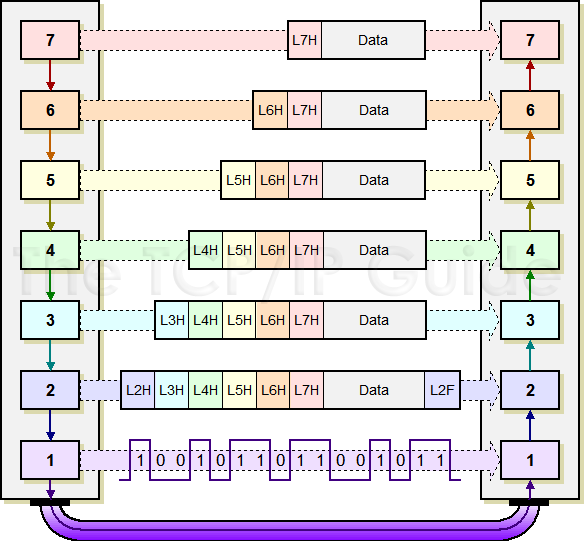
\includegraphics[width=0.4\textwidth]{public/assets/img/osidataenkapsulasi.png}
		\caption{Packet Data Unit}
		\label{fig:pduosi}
	\end{figure}
	\par \textit{Protocol Data Unit} atau dapat disingkat PDU merupakan satuan unit yang ditransmisikan antar \textit{node} pada jaringan. PDU terdiri dari \textit{control information} dan \textit{user data}. Gambar \ref{fig:pduosi} menjelaskan bagaimana PDU berubah di setiap layer.
\end{frame}
\begin{frame}{Intrusion Detection System}
	\begin{figure}
		\centering
		
\includegraphics[width=0.3\textwidth]{public/assets/img/snortlogo.png}
		\caption{Snort IDS}
		\label{fig:snortids}
	\end{figure}
	\par IDS merupakan singkatan dari \textit{Intrusion Detection System}. IDS adalah perangkat atau aplikasi perangkat lunak yang memantau jaringan atau sistem untuk aktivitas jahat atau pelanggaran policy.
	\par Salah satu contoh IDS yang sering digunakan adalah snort IDS yang memiliki logo pada gambar \ref{fig:snortids}. Snort IDS merupakan IDS yang dikembangkan oleh CISCO yang sebelumnya dimiliki oleh Sourcefire. \cite{greenemeier2006sourcefire}
\end{frame}
\begin{frame}{Botnet}
	\par Botnet merupakan sekumpulan program yang saling terhubung dan biasanya mengirimkan pesan spam atau berpartisipasi dalam melakukan DDoS. Botnet menyerang protokol yang menyediakan kanal komunikasi seperti protokol HTTP, IRC, dan Email.
\end{frame}
\begin{frame}{Deep Learning}
	\par Deep learning merupakan salah satu penerapan dari Machine Learning yang digunakan untuk memahami data yang memiliki makna. Contohnya seperti gambar, suara, maupun bentuk data lain yang dapat diinterpretasikan tidak secara matematis. Deep Learning memanfaatkan konsep matematis pada Machine Learning untuk mempelajari data yang lebih kompleks. nyata.\cite{goodfellow2016deep}
\end{frame}
\begin{frame}{Convolutional Neural Network}
	\par CNN merupakan salah satu metode artificial neural network yang biasa diterapkan untuk data dalam bentuk gambar. Pada CNN data gambar melalui proses ekstraksi fitur. Pada proses ekstraksi fitur setiap piksel dari gambar akan diubah dalam bentuk data matriks angka. Fitur yang sudah diekstraksi kemudian akan di alirkan melalui dua layer yaitu \textit{convolutional layer} dan \textit{pooling layer}.
\end{frame}
\begin{frame}{Long Short Term Memory}
	\begin{figure}[H]
		\centering
		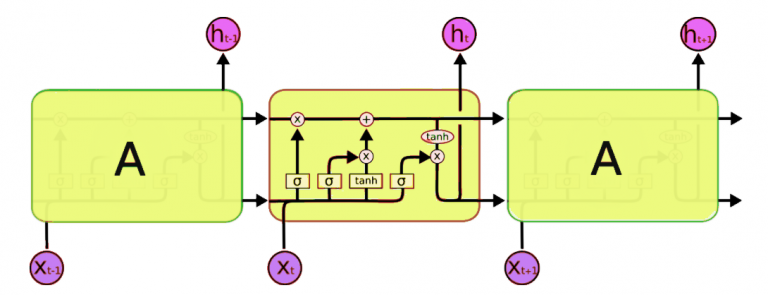
\includegraphics[width=0.8\textwidth]{public/assets/img/LSTM1.png}
		\caption{Layer LSTM}
		\label{fig:lstm1}
	\end{figure}
	\par LSTM (Long short-term memory) memiliki kemampuan untuk melupakan informasi yang tidak relevan pada jaringan RNN (recurrent neural network). LSTM merupakan RNN yang terdiri dari 4 bagian yakni, cell state, input gate, output gate, dan forget gate..
\end{frame}
\begin{frame}{Python}
	\par Python merupakan bahasa pemrograman yang memiliki banyak \textit{library} yang memiliki banyak fungsi dan penerapan. Beberapa \textit{library} python antara lain seperti \textit{tensorflow} dan \textit{keras} yang merupakan framework yang digunakan untuk membuat model jaringan syaraf tiruan maupun \textit{machine learning}.
\end{frame}
\begin{frame}{Flask}
	\par Flask adalah framework web yang dibuat dengan Python. framework ini termasuk dalam kategori \textit{microservice} karena tidak memerlukan \textit{tools} atau \textit{library} tertentu atau dapat juga disebut dengan \textit{microframework}.
\end{frame}
\begin{frame}{Keras}
	\par Keras adalah salah satu library python untuk jaringan syaraf tiruan. Keras merupakan \textit{framework} dari tensorflow, CNTK, atau Theano. Keras dikembangkan sebagai solusi untuk memungkinkan eksperimen jaringan syaraf tiruan dengan cepat. Keras memungkinkan peneliti lebih cepat mengaplikasikan idenya langsung dalam bentuk hasil yang di inginkan.
\end{frame}
\section{Metode Penelitian}
\begin{frame}{Metode Penelitian}
	\begin{figure}[H]
		\centering
		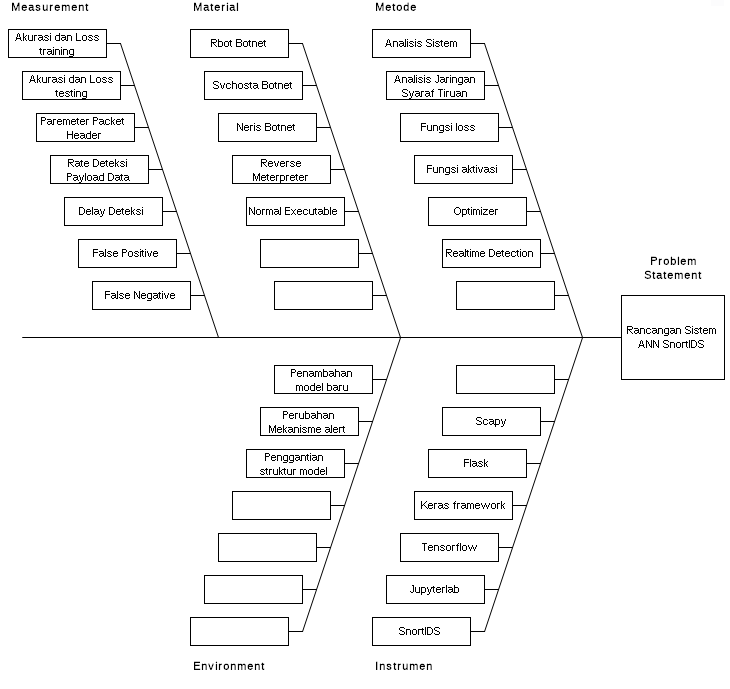
\includegraphics{public/assets/img/fishbonepenelitian.png}
		\caption{Metode Penelitian}
		\label{fig:fishbonepenelitian}
	\end{figure}
\end{frame}
\subsection{Waktu dan Tempat Pelaksanaan}
\begin{frame}{Waktu dan Tempat Pelaksanaan}
	\par Waktu pelaksanaan penelitian dilakukan dari tanggal 1 Maret 2019 sampai dengan 31 September 2019.
	\par Pelaksanaan penelitian dilakukan di Laboratorium 3 UPT Pusat Teknologi Informasi dan Komunikasi Universitas Mataram
\end{frame}
\subsection{Populasi dan Sampel}
\begin{frame}{Populasi dan Sampel}
	\par Populasi pada penelitian ini mencakup intrusi dalam bentuk Executable-based Virus dan Payload-based Virus
	\begin{enumerate}
		\item RBot, Neris, Svchosta Botnet file pcap dan exe
		\item Payload Reverse Meterpreter dalam file PE32
		\item File executable normal
	\end{enumerate}
\end{frame}
\subsection{Instrumen Penelitian}
\begin{frame}{Instrumen Penelitian}
	Instrumen penelitian yang digunakan antara lain :
	\begin{enumerate}
		\item SnortIDS sebagai Intrusion Detection System
		\item Python sebagai bahasa pemrograman yang digunakan untuk pemodelan LSTM dan CNN
		\item Library python seperti : tensorflow, keras, numpy, matplotlib untuk perlengkapan pada saat training data dan testing data dengan Convolutional Neural Network dan Long Short Term Memory.
		\item Python flask sebagai library untuk webservice filter dan profiler
		\item PC Server Linux sebagai host yang menjalankan SnortIDS, dan Python
	\end{enumerate}    
\end{frame}
\subsection{Prosedur Penelitian}
\begin{frame}{Prosedur Penelitian}
	\par Prosedur penelitian terdiri dari perancangan sistem training dan perancangan sistem filter untuk testing. Rancangan sistem training dibuat dengan menggunakan jupyter notebook. Sedangkan rancangan sistem filter menggunakan snortIDS dan flask framework untuk menghubungkan keluaran data dari snortIDS ke dalam model CNN dan LSTM.
\end{frame}
\subsection{Perancangan Sistem}
\begin{frame}{Perancangan Sistem}
	\par Rancangan sistem filter terdiri dari Dataset yang dijadikan data untuk proses testing. Pada sisi filter juga terdapat IP\_buffer yang digunakan sebagai input yang akan mengumpulkan packet yang bersumber dari alamat IP yang sama.
	\par Alamat IP yang berbeda-beda atau berubah-ubah dapat diketahui dari kemiripan transmisi header antara satu packet dengan packet lain. Jika kemiripan nya tinggi maka akan dianggap alamat IP diubah-ubah atau terindikasi Denial of Service.
\end{frame}
\begin{frame}{Perancangan Sistem}
	\begin{figure}[H]
		\centering
		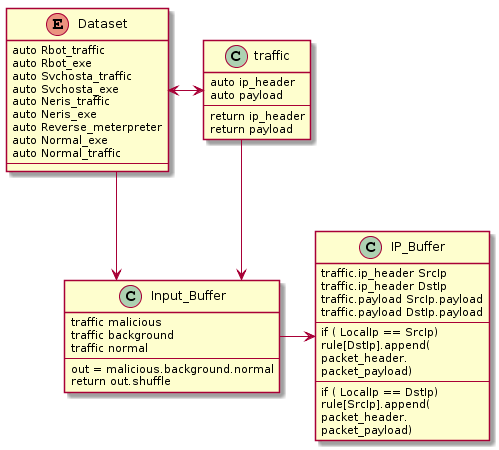
\includegraphics[width=0.6\textwidth]{public/assets/img/RancanganSistemPenelitian.png}
		\caption{Model Rancangan Sistem}
		\label{fig:rancanganpenelitian}
	\end{figure}
\end{frame}
\subsection{Analisis Data}
\begin{frame}{Analisis Data}
	\par Proses analisis data meliputi analisis tabel dan analisis grafis dari seluruh hasil pengujian validitas dan reliabilitas instrumen
	\par Sebelum data dimasukkan, data yang masih mentah diubah menjadi data angka. Pada sistem \textit{profiling}, data angka yang dijadikan input adalah data header yang berisi \textit{IP Address}, \textit{Port} baik sumber maupun tujuan dan beberapa parameter header lainnya. Pada sistem \textit{filtering}, data angka yang dijadikan input diperoleh dari data 1448 byte per frame packet yang diperoleh dari \textit{packet payload}.
	\par Setelah diperoleh data angka pada sistem \textit{profiling} di inputkan data angka header, lalu proses \textit{training} dilakukan untuk memperoleh hasil regresi dari trafik jaringan. Sedangkan pada sistem \textit{filtering} di inputkan data payload yang kemudian akan di lakukan training untuk mengklasifikasi data yang dimasukkan aman atau intrusi. Data hasil training dan testing dari proses ini akan dianalisis untuk menentukan model yang akan digunakan pada sistem pendeteksi intrusi SnortIDS.
\end{frame}
\begin{frame}{Analisis Data}
	\par Analisis data dilakukan berdasarkan dua jenis data yang diperoleh yakni Sistem \textit{Profiling} oleh LSTM, dan Sisitem \textit{Filtering} oleh CNN. Sistem Profiling LSTM menggunakan tiga metode yakni \textit{Sentiment Analysis}, \textit{Multivariate Prediction}, dan \textit{4 Directional Header Prediction}. Ketiga metode ini kemudian masing-masing parameternya akan di analisis agar memperoleh Sistem \textit{Profiling} yang optimal. Sistem Filtering CNN dianalisis dengan mengubah parameter \textit{learning rate}-nya. Dimana \textit{learning rate} yang dipakai adalah 0.1, 0.01, 0.001, dan 0.0001. Hal ini dilakukan untuk mempertimbangkan learning rate yang optimal yang akan digunakan untuk melakukan training model filter.
	\par Untuk menguji analisis payload CNN pada jenis data yang berbeda maka diperlukan beberapa tambahan data lain.
\end{frame}
\begin{frame}{Analisis Data - Data Tambahan}
	\begin{table}[H]
		\centering
		\begin{tabularx}{0.5\textwidth}{|l|X|}
			\hline
			\textbf{Nama Program} & \textbf{Nama File} \\
			\hline
			Calculator            & calc.exe           \\
			\hline
			Cruel game            & cruel.exe          \\
			\hline
			Freecell game         & freecell.exe       \\
			\hline
			Golf game             & golf.exe           \\
			\hline
			MS Paint              & mspaint.exe        \\
			\hline
			Pegged                & pegged.exe         \\
			\hline
			Realterm              & realterm.exe       \\
			\hline
			Reversi game          & reversi.exe        \\
			\hline
			Snake game            & snake.exe          \\
			\hline
			Solitaire game        & sol.exe            \\
			\hline
			Taipei game           & taipei.exe         \\
			\hline
			Winmine game          & winmine.exe        \\
			\hline
		\end{tabularx}
		\caption{Dataset tambahan}
		\label{table:dataset_tambahan}
	\end{table}
\end{frame}
\subsection{Membuat klasifikasi data}
\begin{frame}{Membuat Klasifikasi Data}
	\par Data kelas terbagi menjadi 2 yakni \textit{Malicious} dan \textit{Benign}. Untuk membedakan kedua kelas ini dilakukan training pada data \textit{malicious} dengan dua kelas. Pada sistem filtering klasifikasi terjadi berdasarkan sifat dari payload dari \textit{packet}, sedangkan pada sistem profiling klasifikasi terjadi secara tidak langsung, dengan memperhitungkan anomali trafik jaringan dengan regresi.
\end{frame}
\section{Hasil Penelitian}
\begin{frame}{Hasil Penelitian}
	\par Hasil penelitian meliputi :
	\begin{enumerate}
		\item Data Hasil LSTM dengan metode Sentiment Analysis, Multivariate Prediction, dan 4 Directional Header
		\item Data Hasil CNN dengan variasi ukuran learning-rate
		\item Data Hasil kinerja \textit{Detection Rate} Snort dengan LSTM dan CNN
	\end{enumerate}
\end{frame}
\begin{frame}{LSTM dengan metode Sentiment Analysis}
	\par Untuk Hasil training svchosta dengan sentiment analysis memiliki bentuk sebagai berikut :
	\begin{figure}[H]
		\centering
		\begin{subfigure}[b]{.45\linewidth}
			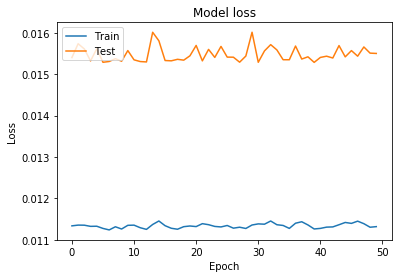
\includegraphics[width=\textwidth]{public/assets/img/lstms_svchosta_loss.png}
		\end{subfigure}
		\begin{subfigure}[b]{.45\linewidth}
			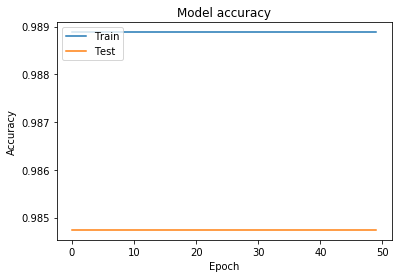
\includegraphics[width=\textwidth] {public/assets/img/lstms_svchosta_acc.png}
		\end{subfigure}
		\caption{Loss dan Akurasi model LSTM svchosta Sentiment Analysis}
		\label{fig:lstms_svchosta}
	\end{figure}
\end{frame}
\begin{frame}{LSTM dengan metode Sentiment Analysis}
	\begin{figure}[H]
		\centering
		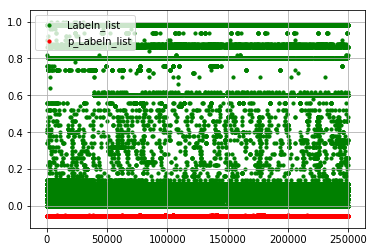
\includegraphics[width=0.5\textwidth]{public/assets/img/lstms_svchosta_pred.png}
		\caption{Hasil Prediksi svchosta Sentiment Analysis}
		\label{fig:lstms_svchosta_pred}
	\end{figure}
	\par Dari kedua gambar \ref{fig:lstms_svchosta} dan gambar \ref{fig:lstms_svchosta_pred}, dapat diamati bahwa tidak ada terjadi proses pembelajaran.
\end{frame}
\begin{frame}{LSTM dengan metode Sentiment Analysis}
    \begin{figure}[H]
        \centering
        \begin{subfigure}[b]{.25\linewidth}
        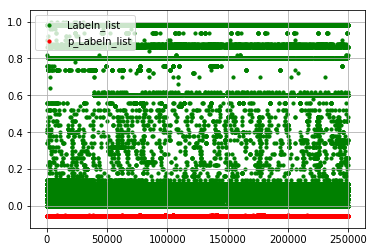
\includegraphics[width=\textwidth]{public/assets/img/lstms_svchosta_pred.png}
        \caption{svchosta}
        \end{subfigure}
        \begin{subfigure}[b]{.25\linewidth}
        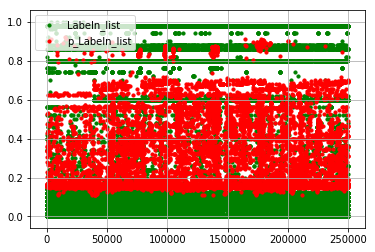
\includegraphics[width=\textwidth]{public/assets/img/lstms_neris_pred.png}
        \caption{neris}
        \end{subfigure}
        \begin{subfigure}[b]{.25\linewidth}
        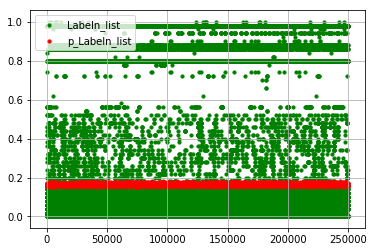
\includegraphics[width=\textwidth]{public/assets/img/lstms_rbot_pred.png}
        \caption{rbot}
        \end{subfigure}
        \caption{Hasil prediksi dengan sentiment Analysis}
        \label{fig:lstmss_pred}
    \end{figure}
    \par Dapat diamati dari gambar \ref{fig:lstmss_pred} bahwa titik prediksi tidak sesuai dengan titik trafik asli. Hal ini dikarenakan sedikitnya trafik yang membedakan trafik malware dan normal.
\end{frame}
\begin{frame}{LSTM dengan metode Multivariate Prediction}
	\begin{figure}[H]
		\centering
		\begin{subfigure}[b]{.45\linewidth}
		    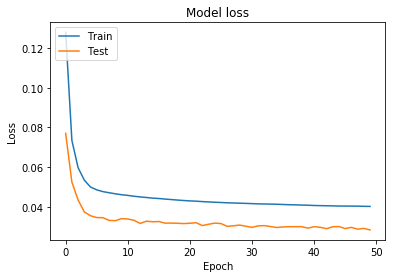
\includegraphics[width=\textwidth]{public/assets/img/lstmm_svchosta_loss.png}
		    \caption{Loss}
		\end{subfigure}
		\begin{subfigure}[b]{.45\linewidth}
		    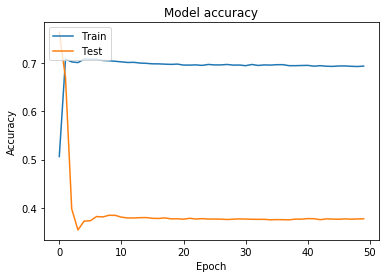
\includegraphics[width=\textwidth]{public/assets/img/lstmm_svchosta_acc.png}
		    \caption{Accuracy}
		\end{subfigure}
		\caption{Loss dan Akurasi model LSTM svchosta Multivariate Prediction}
		\label{fig:lstmm_svchosta}
	\end{figure}
	\per Berdasarkan grafik \ref{fig:lstmm_svchosta} diatas, kita dapat amati bahwa terjadi proses pembelajaran.
\end{frame}
\begin{frame}{LSTM Multivariate Prediction svchosta}
    \begin{subfigure}[b]{0.3\linewidth}
        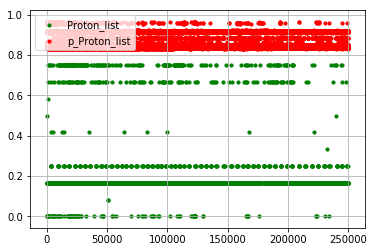
\includegraphics[width=\textwidth]{public/assets/img/lstmm_svchosta_pred1.png}
    \end{subfigure}
    \begin{subfigure}[b]{0.3\linewidth}
        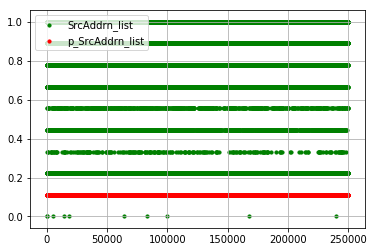
\includegraphics[width=\textwidth]{public/assets/img/lstmm_svchosta_pred2.png}
    \end{subfigure}
       \begin{subfigure}[b]{0.3\linewidth}
        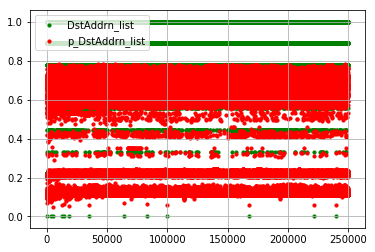
\includegraphics[width=\textwidth]{public/assets/img/lstmm_svchosta_pred3.png}
    \end{subfigure}
    \begin{subfigure}[b]{0.3\linewidth}
        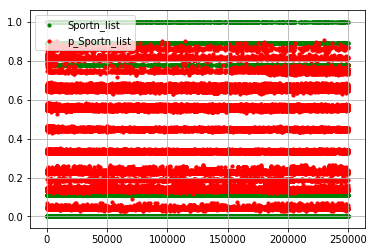
\includegraphics[width=\textwidth]{public/assets/img/lstmm_svchosta_pred4.png}
    \end{subfigure}
    \begin{subfigure}[b]{0.3\linewidth}
        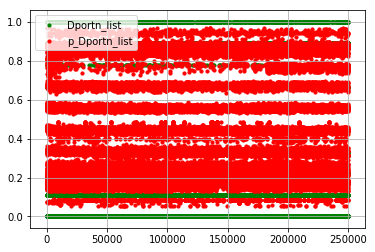
\includegraphics[width=\textwidth]{public/assets/img/lstmm_svchosta_pred5.png}
    \end{subfigure}
    \begin{subfigure}[b]{0.3\linewidth}
        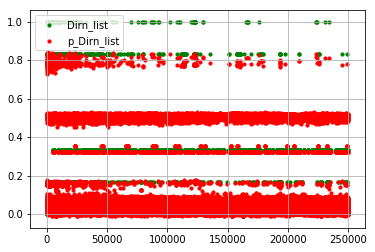
\includegraphics[width=\textwidth]{public/assets/img/lstmm_svchosta_pred6.png}
    \end{subfigure}
    \begin{subfigure}[b]{0.3\linewidth}
        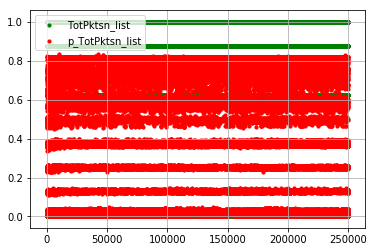
\includegraphics[width=\textwidth]{public/assets/img/lstmm_svchosta_pred7.png}
    \end{subfigure}
    \begin{subfigure}[b]{0.3\linewidth}
        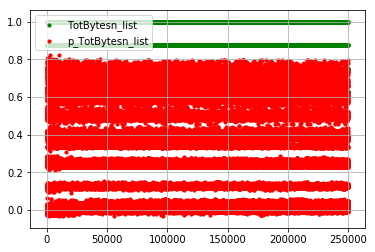
\includegraphics[width=\textwidth]{public/assets/img/lstmm_svchosta_pred8.png}
    \end{subfigure}
    \begin{subfigure}[b]{0.3\linewidth}
        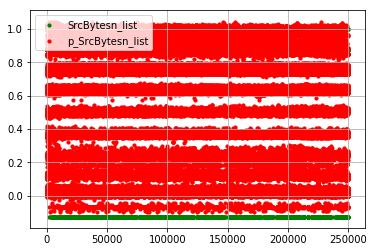
\includegraphics[width=\textwidth]{public/assets/img/lstmm_svchosta_pred9.png}
    \end{subfigure}
\end{frame}
\begin{frame}{LSTM dengan metode 4 Directional Header}
   \begin{figure}[H]
   \begin{subfigure}[b]{.45\linewidth}
        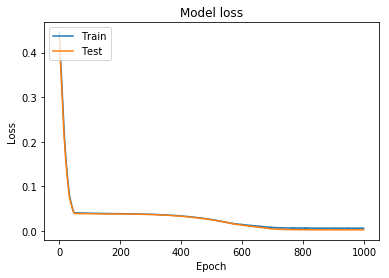
\includegraphics[width=\textwidth]{public/assets/img/lstm4_svchosta_loss.png}
        \caption{Loss}
   \end{subfigure}
   \begin{subfigure}[b]{.45\linewidth}
        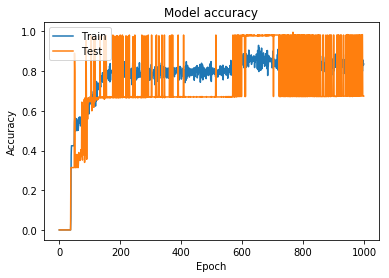
\includegraphics[width=\textwidth]{public/assets/img/lstm4_svchosta_acc.png}
        \caption{Akurasi}
   \end{subfigure}
   \caption{Loss dan Akurasi model LSTM svchosta 4 Directional Header}
   \label{fig:lstm4_svchosta}
   \end{figure}
   \par Berdasarkan gambar \ref{fig:lstm4_svchosta}, dapat diamati pada model ini terjadi proses pembelajaran. Pada sisi loss dapat diamati hasil training dan testing berhimpitan menandakan kecocokan hasil training dan testing yang tinggi.
\end{frame}
\begin{frame}{LSTM dengan metode 4 Directional Header | Prediksi}
    \begin{figure}[H]
    \begin{subfigure}[b]{.35\linewidth}
        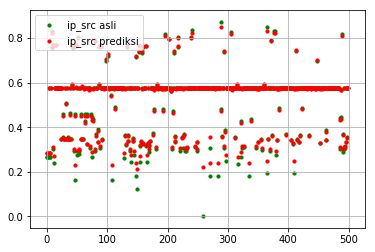
\includegraphics[width=\textwidth]{public/assets/img/lstm4_svchosta_pred1.png}
        \caption{IPSrc}
    \end{subfigure}
    \begin{subfigure}[b]{.35\linewidth}
        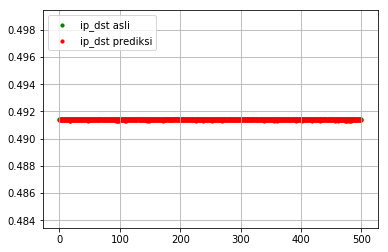
\includegraphics[width=\textwidth]{public/assets/img/lstm4_svchosta_pred2.png}
        \caption{IPDst}
    \end{subfigure}
    \begin{subfigure}[b]{.35\linewidth}
        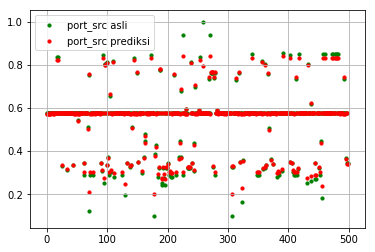
\includegraphics[width=\textwidth]{public/assets/img/lstm4_svchosta_pred3.png}
        \caption{PortSrc}
    \end{subfigure}
    \begin{subfigure}[b]{.35\linewidth}
        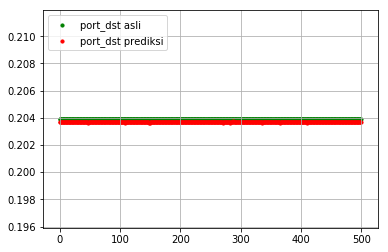
\includegraphics[width=\textwidth]{public/assets/img/lstm4_svchosta_pred4.png}
        \caption{PortDst}
    \end{subfigure}
    \end{figure}
\end{frame}
\begin{frame}{LSTM Summary}
    \par Berdasarkan ketiga metode yang digunakan di LSTM dapat dijabarkan perbedaannya sebagai berikut.
    \begin{table}[H]
    \begin{tabularx}{\textwidth}{
                |c
                |p{0.6\textwidth}|}
    \hline
    \thead{Metode} & \thead{Karakteristik} \\
    \hline
    Sentiment Analysis & Tidak konvergen, sehingga tidak perlu dilanjutkan \\
    \hline
    Multivariate Prediction & Konvergen, tetapi banyak parameter yang mengganggu proses training \\
    \hline
    4 Directional Header & Konvergen dan karena hanya menggunakan bagian yang benar-benar diperhitungkan sehingga hasil yang diperoleh akurat \\
    \hline
    \end{tabularx}
    \caption{Data hasil perbandingan metode LSTM}
    \label{table:data_perbandingan_lstm}
    \end{table}
\end{frame}
\begin{frame}{CNN | Loss dan Akurasi}
    \begin{figure}[H]
    \begin{subfigure}[b]{.45\linewidth}
        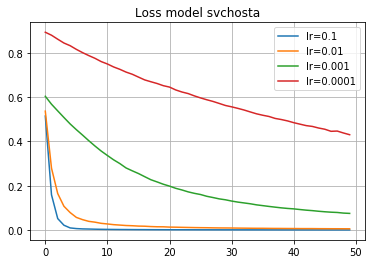
\includegraphics[width=\textwidth]{public/assets/img/cnn_svchosta_loss.png}
        \caption{Loss}
    \end{subfigure}
    \begin{subfigure}[b]{.45\linewidth}
        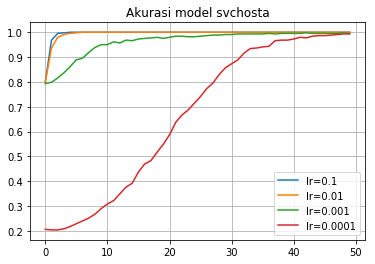
\includegraphics[width=\textwidth]{public/assets/img/cnn_svchosta_acc.png}
        \caption{Akurasi}
    \end{subfigure}
    \caption{Loss dan Akurasi CNN}
    \label{fig:cnn_svchosta}
    \end{figure}
    \par Dari gambar \ref{fig:cnn_svchosta} diatas, dapat kita amati perbedaan proses training CNN ketika ukuran learning rate nya diubah-ubah.
\end{frame}
\begin{frame}{CNN | Hasil Prediksi}
\begin{figure}[H]
    \begin{subfigure}[b]{.23\linewidth}
        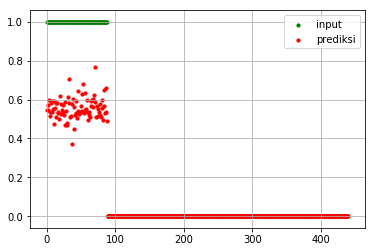
\includegraphics[width=\textwidth]{public/assets/img/cnn_svchosta_train_pred01.png}
        \caption{lr=0.1} 
    \end{subfigure}
    \begin{subfigure}[b]{.23\linewidth}
        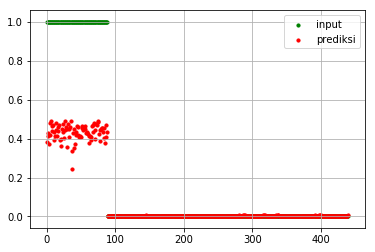
\includegraphics[width=\textwidth]{public/assets/img/cnn_svchosta_train_pred001.png}
        \caption{lr=0.01}
    \end{subfigure}
    \begin{subfigure}[b]{.23\linewidth}
        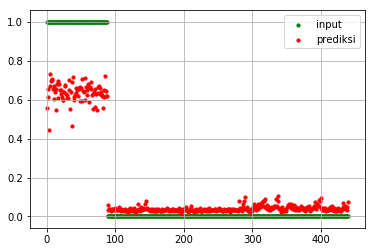
\includegraphics[width=\textwidth]{public/assets/img/cnn_svchosta_train_pred0001.png}
        \caption{lr=0.001}
    \end{subfigure}
    \begin{subfigure}[b]{.23\linewidth}
        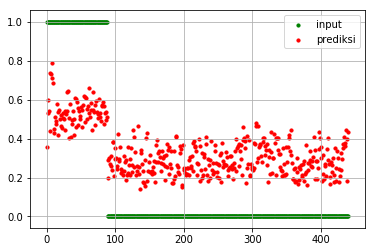
\includegraphics[width=\textwidth]{public/assets/img/cnn_svchosta_train_pred00001.png}
        \caption{lr=0.0001}
    \end{subfigure}
\end{figure}
\begin{figure}[H]
    \begin{subfigure}[b]{.23\linewidth}
        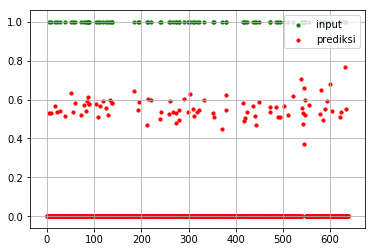
\includegraphics[width=\textwidth]{public/assets/img/cnn_svchosta_test_pred01.png}
        \caption{lr=0.1}
    \end{subfigure}
    \begin{subfigure}[b]{.23\linewidth}
        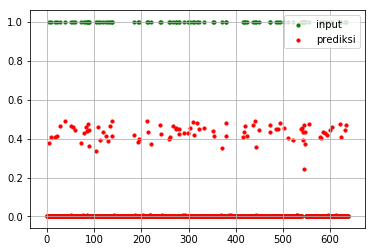
\includegraphics[width=\textwidth]{public/assets/img/cnn_svchosta_test_pred001.png}
        \caption{lr=0.01}
    \end{subfigure}
    \begin{subfigure}[b]{.23\linewidth}
        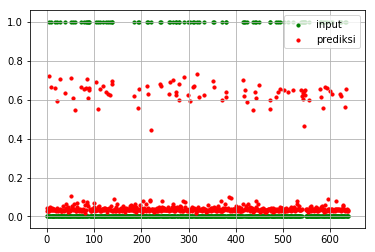
\includegraphics[width=\textwidth]{public/assets/img/cnn_svchosta_test_pred0001.png}
        \caption{lr=0.001}
    \end{subfigure}
    \begin{subfigure}[b]{.23\linewidth}
        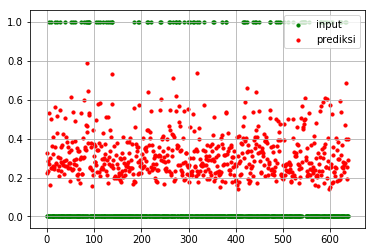
\includegraphics[width=\textwidth]{public/assets/img/cnn_svchosta_test_pred00001.png}
        \caption{lr=0.0001}
    \end{subfigure}
\end{figure}
\end{frame}
\begin{frame}{Detection Rate}
\begin{table}[H]
\centering
\begin{tabularx}{0.9\textwidth}{|*{6}{Y|}}
\hline
    \multirow{2}{*}{Dataset} 
  & \multirow{2}{*}{Ukuran}
  & \multicolumn{3}{c|}{Runtime}
  & \multirow{2}{*}{Detection} \\
\cline{3-5}
 & Paket & Snort (s) & LSTM (s) & CNN (s) & Rate (p/s)\\
\hline
svchosta & 185 & 0.1047 & 0.7968 & 19.4115 & 9.1074\\
neris & 652 & 1.5970 & 0.4882 & 81.2973 & 7.8193\\
rbot & 278 & 1.2519 & 0.3975 & 35.0600 & 7.5729\\
\hline
\end{tabularx}
\caption{Data hasil detection rate preprocessor}
\label{table:detection_rate}
\end{table}
\par Berdasarkan tabel \ref{table:detection_rate} dapat diamati bahwa packet terbesar yang dianalisis dari neris sebesar 652 memiliki Detection Rate sekitar 7.8193 paket per detik. Detection rate tertinggi pada svchosta mencapai 9.1074 paket per detik.
\end{frame}
\section{DEMO}
\begin{frame}{DEMO}
\centering
    \Large DEMO
\end{frame}
\section{Penutup}
\begin{frame}{Penutup}
	Kesimpulan :
	\begin{enumerate}
		\item Hasil yang diperoleh pada metode LSTM untuk proses profiling trafik yang terbaik diperoleh dengan menggunakan metode 4 directional header, dapat dilihat dari konvergensi dan ketepatan prediksi data dengan input data.
		\item Hasil yang diperoleh pada metode CNN untuk proses filtering payload memiliki pola semakin tinggi learning rate yang digunakan maka konvergensi atau peningkatan akurasi dan pengurangan loss terjadi lebih cepat beberapa epoch dari learning rate yang rendah.
		\item Hasil detection rate dengan snort diperoleh kinerja tertinggi pendeteksian dengan detection rate tertinggi pada paket svchosta dengan kecepatan 9.1074 paket per detik.
	\end{enumerate}
\end{frame}
\begin{frame}{Penutup}
	Saran :
	\begin{enumerate}
		\item Agar integrasi Sistem Pendeteksi Intrusi Snort dan Keras framework dapat dioptimasi sehingga pendeteksian dapat terjadi dengan cepat atau mendekati realtime. Penelitian sebaiknya dilakukan dengan hardware yang memiliki daya komputasi yang kuat.
		\item Agar mekanisme Sistem Pendeteksi Intrusi dapat diterapkan secara portabel, perlu adanya sistem yang dapat mengkonversi dari satu model dengan backend lain selain keras
	\end{enumerate}
\end{frame}
\section{Daftar Pustaka}
\begin{frame}[t, allowframebreaks]
	\frametitle{Daftar Pustaka}
	\bibliographystyle{agsm}
	\bibliography{skripsi}
\end{frame}
\end{document}